% Hlavicka pro protokoly z fyzikalniho praktika.
% Verze pro: LaTeX
% Verze hlavicky: 22. 2. 2007
% Autor: Ustav fyziky kondenzovanych latek
% Ke stazeni: www.physics.muni.cz/ufkl/Vyuka/
% Licence: volne k pouziti, nejlepe k vcasnemu odevzdani protokolu z Vaseho mereni.


\documentclass[czech,11pt,a4paper]{article}
\usepackage[T1]{fontenc}
\usepackage{graphicx, animate}
\usepackage{mathtools}
\usepackage{amssymb}
\usepackage{amsthm}
\usepackage{thmtools}
\usepackage{xcolor}
\usepackage{nameref}
\usepackage{babel}
\usepackage{hyperref}
\usepackage{multicol}
\usepackage[export]{adjustbox}
\usepackage{subcaption}
\usepackage{caption}
\usepackage{multirow}
\usepackage{float}
\usepackage{placeins}
\usepackage{biblatex}
\graphicspath{ {./images/} }




%%% Nemente:
\usepackage[margin=2cm]{geometry}
\newtoks\jmenopraktika \newtoks\jmeno \newtoks\datum
\newtoks\obor \newtoks\skupina \newtoks\rocnik \newtoks\semestr
\newtoks\cisloulohy \newtoks\jmenoulohy
\newtoks\tlak \newtoks\teplota \newtoks\vlhkost
%%% Nemente - konec.


%%%%%%%%%%% Doplnte pozadovane polozky:

\jmenopraktika={Fyzikální praktikum 2}  % nahradte jmenem vaseho predmetu
\jmeno={Teodor Duraković}            % nahradte jmenem mericiho
\datum={18.~listopadu 2024}        % nahradte datem mereni ulohy
\obor={F}                     % nahradte zkratkou vami studovaneho oboru
\skupina={Po 14:00}            % nahradte dobou vyuky vasi seminarni skupiny
\rocnik={II}                  % nahradte rocnikem, ve kterem studujete
\semestr={III}                 % nahradte semestrem, ve kterem studujete

\cisloulohy={7}               % nahradte cislem merene ulohy
\jmenoulohy={Fresnelovy koeficienty, index lomu} % nahradte jmenem merene ulohy

\tlak={983}                   % nahradte tlakem pri mereni (v hPa)
\teplota={21.8}               % nahradte teplotou pri mereni (ve stupnich Celsia)
\vlhkost={35}               % nahradte vlhkosti vzduchu pri mereni (v %)

%%%%%%%%%%% Konec pozadovanych polozek.


%%%%%%%%%%% Uzitecne balicky:

%%%%%% Zamezeni parchantu:
\widowpenalty 10000 \clubpenalty 10000 \displaywidowpenalty 10000
%%%%%% Parametry pro moznost vsazeni vetsiho poctu obrazku na stranku
\setcounter{topnumber}{3}	  % max. pocet floatu nahore (specifikace t)
\setcounter{bottomnumber}{3}	  % max. pocet floatu dole (specifikace b)
\setcounter{totalnumber}{6}	  % max. pocet floatu na strance celkem
\renewcommand\topfraction{0.9}	  % max podil stranky pro floaty nahore
\renewcommand\bottomfraction{0.9} % max podil stranky pro floaty dole
\renewcommand\textfraction{0.1}	  % min podil stranky, ktery musi obsahovat text
\intextsep=8mm \textfloatsep=8mm  %\intextsep pro ulozeni [h] floatu a \textfloatsep pro [b] or [t]

% Tecky za cisly sekci:
\renewcommand{\thesection}{\arabic{section}.}
\renewcommand{\thesubsection}{\thesection\arabic{subsection}.}
\renewcommand{\thesubsubsection}{\thesubsection\arabic{subsubsection}.}
% Jednopismenna mezera mezi cislem a nazvem kapitoly:
\makeatletter \def\@seccntformat#1{\csname the#1\endcsname\hspace{1ex}} \makeatother


%%%%%%%%%%%%%%%%%%%%%%%%%%%%%%%%%%%%%%%%%%%%%%%%%%%%%%%%%%%%%%%%%%%%%%%%%%%%%%%
%%%%%%%%%%%%%%%%%%%%%%%%%%%%%%%%%%%%%%%%%%%%%%%%%%%%%%%%%%%%%%%%%%%%%%%%%%%%%%%
% Zacatek dokumentu
%%%%%%%%%%%%%%%%%%%%%%%%%%%%%%%%%%%%%%%%%%%%%%%%%%%%%%%%%%%%%%%%%%%%%%%%%%%%%%%
%%%%%%%%%%%%%%%%%%%%%%%%%%%%%%%%%%%%%%%%%%%%%%%%%%%%%%%%%%%%%%%%%%%%%%%%%%%%%%%

\begin{document}
	
	%%%%%%%%%%%%%%%%%%%%%%%%%%%%%%%%%%%%%%%%%%%%%%%%%%%%%%%%%%%%%%%%%%%%%%%%%%%%%%%
	% Nemente:
	%%%%%%%%%%%%%%%%%%%%%%%%%%%%%%%%%%%%%%%%%%%%%%%%%%%%%%%%%%%%%%%%%%%%%%%%%%%%%%%
	\thispagestyle{empty}
	
	{
		\begin{center}
			\sf 
			{\Large Ústav fyzikální elektroniky Přírodovědecké fakulty Masarykovy univerzity} \\
			\bigskip
			{\huge \bfseries FYZIKÁLNÍ PRAKTIKUM} \\
			\bigskip
			{\Large \the\jmenopraktika}
		\end{center}
		
		\bigskip
		
		\sf
		\noindent
		\setlength{\arrayrulewidth}{1pt}
		\begin{tabular*}{\textwidth}{@{\extracolsep{\fill}} l l}
			\large {\bfseries Zpracoval:}  \the\jmeno & \large  {\bfseries Naměřeno:} \the\datum\\[2mm]
			\large  {\bfseries Obor:} \the\obor  \hspace{40mm}  {\bfseries Skupina:} \the\skupina %
			%{\bfseries Ročník:} \the\rocnik \hspace{5mm} {\bfseries Semestr:} \the\semestr  
			&\large {\bfseries Testováno:}\\
			\\
			\hline
		\end{tabular*}
	}
	
	\bigskip
	
	{
		\sf
		\noindent \begin{tabular}{p{3cm} p{0.6\textwidth}}
			\Large  Úloha č. {\bfseries \the\cisloulohy:} \par
			\smallskip
			$T=\the\teplota$~$^\circ$C \par
			$p=\the\tlak$~hPa \par
			$\varphi=\the\vlhkost$~\%
			&\Large \bfseries \the\jmenoulohy  \\[2mm]
		\end{tabular}
	}
	
	\vskip1cm
	
	%%%%%%%%%%%%%%%%%%%%%%%%%%%%%%%%%%%%%%%%%%%%%%%%%%%%%%%%%%%%%%%%%%%%%%%%%%%%%%%
	% konec Nemente.
	%%%%%%%%%%%%%%%%%%%%%%%%%%%%%%%%%%%%%%%%%%%%%%%%%%%%%%%%%%%%%%%%%%%%%%%%%%%%%%%
	
	%%%%%%%%%%%%%%%%%%%%%%%%%%%%%%%%%%%%%%%%%%%%%%%%%%%%%%%%%%%%%%%%%%%%%%%%%%%%%%%
	%%%%%%%%%%%%%%%%%%%%%%%%%%%%%%%%%%%%%%%%%%%%%%%%%%%%%%%%%%%%%%%%%%%%%%%%%%%%%%%
	% Zacatek textu vlastniho protokolu
	%%%%%%%%%%%%%%%%%%%%%%%%%%%%%%%%%%%%%%%%%%%%%%%%%%%%%%%%%%%%%%%%%%%%%%%%%%%%%%%
	%%%%%%%%%%%%%%%%%%%%%%%%%%%%%%%%%%%%%%%%%%%%%%%%%%%%%%%%%%%%%%%%%%%%%%%%%%%%%%%
	
	\begin{multicols}{2}
		\section{Zadání}
		
		\section*{Měření odrazivosti dielektrika}
		\section*{Teorie}
		Chování elektromagnetické světelné vlny při odrazu (nebo lomu) na rozhraní dvou neabsorbujících prostředí zjistíme z Maxwellových rovnic. Situace je znázorněna na obr. 1. Rovina dopadu je definována dopadajícím paprskem světla s vlnovým vektorem $\boldsymbol{k}_{0}$ a kolmicí $\boldsymbol{s}$ k uvažovanému rozhraní dvou dielektrických prostředí. $\boldsymbol{E}_{0}$ a $\boldsymbol{E}_{R}$ jsou amplitudy dopadající a odražené vlny, přičemž $p$ a $s$ jsou složky amplitudy lineárně polarizovaného světla rovnoběžné s rovinou dopadu resp. kolmé k této rovině. Symbolem $n_{0}$ je označen index lomu okolního prostředí (vzduch), $n$ je index lomu měřeného dielektrika. Řešením vlnové rovnice dostáváme pro odraženou vlnu s vlnovým\\
		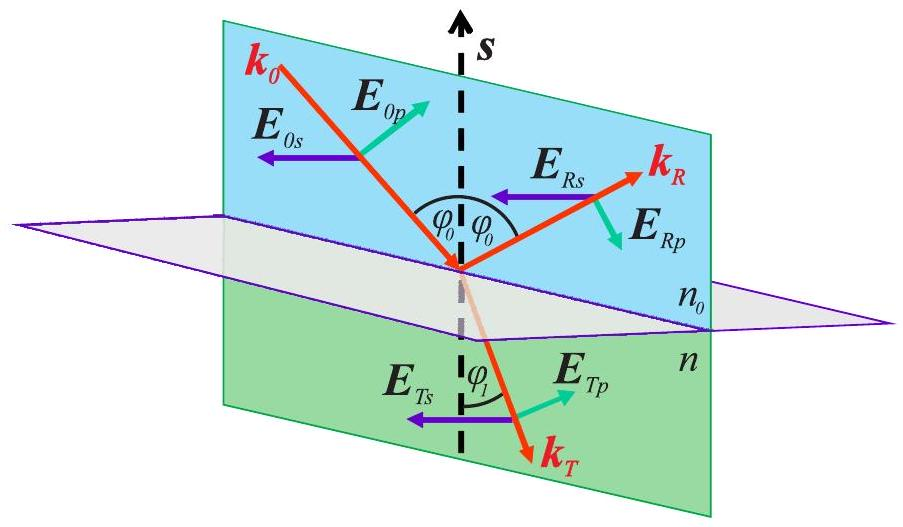
\includegraphics[max width=0.95\linewidth, center]{2024_11_19_160a1389244899f42734g-1}
		
		Obrázek 1: Rozklad amplitudy elektromagnetické vlny do s- a p-polarizace při odrazu na rozhraní.\\
		vektorem $\boldsymbol{k}_{R}$ Fresnelovy amplitudy $r_{p}$ a $r_{s}\left(r_{p}=\left|\boldsymbol{E}_{R p}\right| /\left|\boldsymbol{E}_{0 p}\right|, r_{s}=\left|\boldsymbol{E}_{R s}\right| /\left|\boldsymbol{E}_{0 s}\right| ; \boldsymbol{E}_{R s}\right.$ a $\boldsymbol{E}_{0 s}$ jsou kolmé k rovině dopadu a $\boldsymbol{E}_{R p}$ a $\boldsymbol{E}_{0 p}$ leží v rovině dopadu), které jsou dány vztahy
		
		\begin{equation}
			r_{p}=-\frac{\tan \left(\varphi_{0}-\varphi_{1}\right)}{\tan \left(\varphi_{0}+\varphi_{1}\right)} \quad r_{s}=-\frac{\sin \left(\varphi_{0}-\varphi_{1}\right)}{\sin \left(\varphi_{0}+\varphi_{1}\right)}
		\end{equation}
		
		
		kde úhel $\varphi_{0}$ je úhel dopadu světelného paprsku na rozhraní a $\varphi_{1}$ označuje úhel lomu lomeného paprsku s vlnovým vektorem $\boldsymbol{k}_{T}$. Tyto úhly souvisí prostřednictvím Snellova zákona
		
		\begin{equation}
			n_{0} \sin \varphi_{0}=n_{1} \sin \varphi_{1}
		\end{equation}
		
		
		Na základě Snellova zákona (2) je možné vztahy (1) přepsat do tvaru
		
		
		\begin{equation}
			r_{p}=\frac{n_{0} \cos \varphi_{1}-n \cos \varphi_{0}}{n_{0} \cos \varphi_{1}+n \cos \varphi_{0}} \quad r_{s}=\frac{n_{0} \cos \varphi_{0}-n \cos \varphi_{1}}{n_{0} \cos \varphi_{0}+n \cos \varphi_{1}}
		\end{equation}
		
		Z této dvojice vztahů je zřejmé, že amplitudy $\boldsymbol{E}_{R p, s}$ jsou závislé na úhlu dopadu $\varphi_{0}$ světelného paprsku a na indexech lomu obou prostředí. Rozbor vztahu 1 ukazuje, že při šíření světla z prostředí opticky řidšího do opticky hustšího $\left(n_{0}<n\right)$ je amplituda $r_{s}<0$ pro všechny úhly dopadu, zatímco $r_{p}<0$ pro $\varphi<\varphi_{B}$ a $r_{p}>0$ pro $\varphi>\varphi_{B}$, kde $\varphi_{B}$ je tzv. polarizační (Brewsterův) úhel, pro nějž je $r_{p}=0{ }^{1}$ Tento fakt je významný pro optickou praxi. V tomto případě se totiž odráží pouze s-složka lineárně polarizovaného světla. To platí i pro odraz přirozeného světla a proto lze odrazem na povrchu dielektrického zrcadla při polarizačním úhlu dosáhnout lineárně polarizované vlny. Je-li $r_{p}=0$, pak jmenovatel v prvním vztahu 1. roste do nekonečna, tedy $\varphi_{0}+\varphi_{1}=\pi / 2$; paprsek odražený a lomený jsou navzájem kolmé. Ze vztahu 7.3 pro $r_{p}=0$, dostáváme matematický zápis Brewsterova zákona
		
		\begin{equation}
			\tan \varphi_{B}=n
		\end{equation}
		
		
		pokud $n_{0}=1$.\\
		 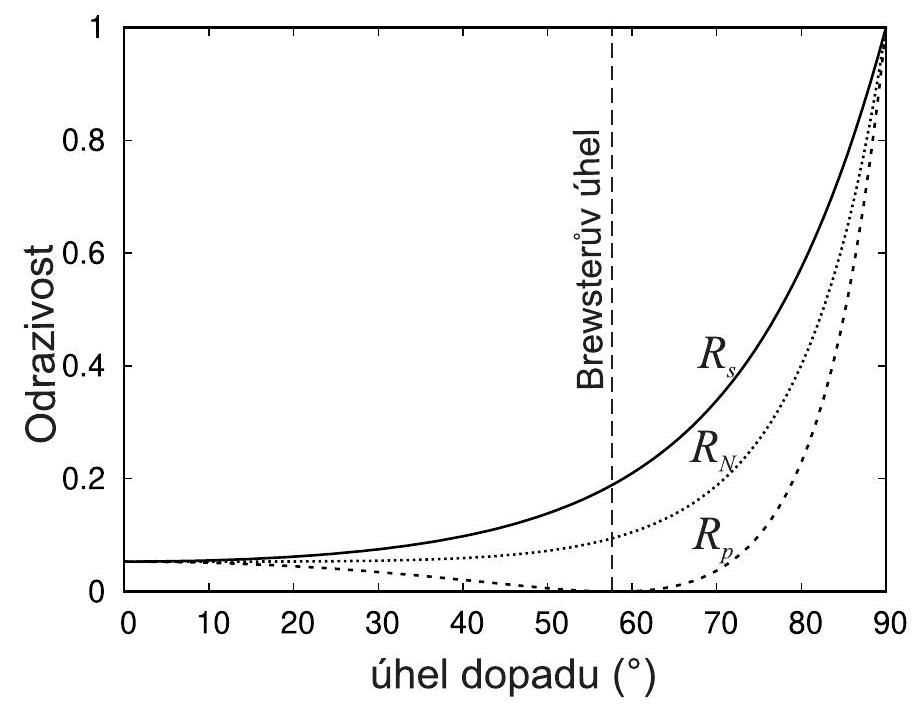
\includegraphics[max width=0.95\linewidth, center]{2024_11_19_160a1389244899f42734g-2}
		
		Obrázek 2: Závislost odrazivosti s-polarizované $\left(R_{s}\right)$ a p-polarizované $\left(R_{p}\right)$ vlny na úhlu odrazu podle Fresnelových vztahů na prostředí s indexem lomu $n=1,6$. Odrazivost nepolarizovaného světla $\left(R_{N}\right)$.
		
		\footnotetext{${ }^{1}$ Záporné hodnoty amplitud znamenají fázový posuv o $\pi$. Je-li $r_{p}>0$ a $r_{s}<0$, je složka $r_{s}$ posunuta o $\pi$ proti složce $r_{p}$. Je-li $r_{p}<0$ a $r_{s}<0$, mají sice obě fázový posuv o $\pi$, ale jejich fázový rozdíl je 0 nebo $2 \pi$.
		}Je-li intenzita složek dopadajícího světla $I_{p}^{0}$ a $I_{s}^{0}$ a intenzita odraženého světla pro obě složky $I_{p}^{R}$ a $I_{s}^{R}$, pak definujeme odrazivosti $R_{p}$ a $R_{s}$ jako
		
		
		\begin{equation}
			R_{p}=\frac{I_{p}^{R}}{I_{p}^{0}} \quad R_{s}=\frac{I_{s}^{R}}{I_{p}^{0}}
		\end{equation}
		
		Odrazivosti jsou pak dány vztahy
		
\begin{equation}
			R_{p}=r_{p}^{2} \quad R_{s}=r_{s}^{2}
\end{equation}
		
		
		Závislosti $R_{p}$ a $R_{s}$ na úhlu dopadu mají odlišný charakter (viz obr. 2). Veličina $R_{s}$ monotonně roste s rostoucí hodnotou $\varphi_{0}$, a při úhlu dopadu 90 stupňǔ je rovná jedné. Odrazivost $R_{p} \mathrm{~s}$ rostoucí hodnotou úhlu dopadu nejprve klesá k nule, při $\varphi_{0}=\varphi_{B}$ je $R_{p}=0$ a pro $\varphi_{0}>\varphi_{B}$ opĕt rychle roste: pro 90 stupňú je opět $R_{p}=1$. Odrazivost přirozeného světla odraženého na rozhraní dvou neabsorbujících prostředí je pak dána vztahem
		
		
\begin{equation}
			R_{N}=R_{s} / 2+R_{p} / 2
\end{equation}
		
		
		Z odrazivostí $R_{p}$ a $R_{s}$ jsme také schopni stanovit hodnoty indexu lomu méřeného dielektrika. Výrazy $\pm \sqrt{R_{p}}$ a $\pm \sqrt{R_{s}}$ odpovídají pravé straně vztahů $\sqrt{3}$, přičemž znaménko plus nebo mínus před odmocninou je dáno v každém konkrétním případĕ fyzikální podstatou problému. Za předpokladu, že se měření provádí ve vzduchu, platí $n_{0}=1$ a můžeme např. z prvního vztahu (7.3) vypočítat $\cos \varphi_{1}$ a dosadit jej do druhého vztahu (3). Jednoduchou úpravou pak dostaneme za předpokladu, že provádíme mĕření na skle, následující vztahy pro hledaný index lomu skla: pro úhly dopadu $\varphi_{0}<\varphi_{B}$ platí
		
		
		\begin{equation}
			n=\sqrt{\frac{\left(1+\sqrt{R_{s}}\right)\left(1+\sqrt{R_{p}}\right)}{\left(1-\sqrt{R_{s}}\right)\left(1-\sqrt{R_{p}}\right)}}
		\end{equation}
		
		pro případ $\varphi_{0}>\varphi_{B}$ pak
		
		
		\begin{equation}
			n=\sqrt{\frac{\left(1+\sqrt{R_{s}}\right)\left(1-\sqrt{R_{p}}\right)}{\left(1-\sqrt{R_{s}}\right)\left(1+\sqrt{R_{p}}\right)}}
		\end{equation}
		
		Tento postup v sobě skrývá určitou potíž spočívající v tom, že výpočet indexu lomu je v tomto případě založen na znalosti absolutních hodnot odrazivosti p- a s- složky lineárně polarizovaného světla.
		
		\section{Experiment}
		Smyslem této úlohy je zjistit průběh křivek $R_{p}=f\left(\varphi_{0}\right)$ a $R_{s}=f\left(\varphi_{0}\right)$ pro danou neabsorbující látku a využitím vztahu (7.4) určit pro použitou vlnovou délku světla index lomu dané látky. Principiální uspořádání experimentu je uvedeno na obr. 3 úzký svazek paprsků vycházející z laseru ( L ) prochází polarizátorem ( P ). Zde se světlo lineárně polarizuje a otáčením polarizátoru lze docílit toho, že kmitová rovina je rovnoběžná (kolmá) s rovinou dopadu, což odpovídá p- (s-) složce amplitudy dopadajícího světla. Po odrazu světla na měřeném vzorku umístěném na stolečku goniometru svazek světla dopadá na detektor (D) spojený s měřícím přístrojem. Otáčením stolečku se vzorkem kolem jeho svislé osy měníme úhel dopadu $\varphi_{0}$ světelného svazku a odečítáme signál na měřicím přístroji detektoru (ampérmetru). Chceme-li určit úhlovou závislost odrazivosti $R_{p}$ a $R_{s}$, je třeba před začátkem měření odstranit ze stolečku  vzorek a v místě označeném (A) detektorem stanovit intenzitu dopadajícího svazku $I_{s}^{0}$ a $I_{p}^{0}$. Odrazivosti odraženého světla $R_{p}$ a $R_{s}$ pak vyjádříme jako
		
		\begin{equation}
			R_{p}=\frac{I_{p}^{R}}{I_{p}^{0}} \quad R_{s}=\frac{I_{s}^{R}}{I_{s}^{0}}
		\end{equation}
		
		kde $I_{p}^{R}$ a $I_{s}^{R}$ jsou $s$ a $p$ polarizované intenzity odraženého záření.
		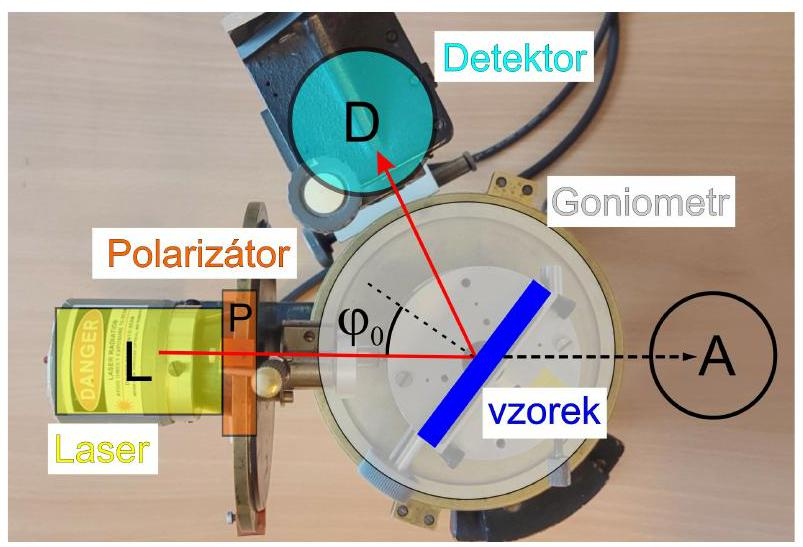
\includegraphics[max width=0.9\linewidth, center]{2024_11_19_160a1389244899f42734g-4}
		
		Obrázek 3: Experimentální uspořádání pro měření úhlové závislosti odrazivosti dielektrika. Poloha detektoru A odpovídá referenční pozici pro měření signálu bez vzorku.
		
		\section*{Úkoly}
		\begin{enumerate}
			\item Stanovte úhlové závislosti odrazivosti $R_{p}, R_{s}$ lineárně polarizovaného světla pro danou látku.
			\item Určete hodnotu Brewsterova úhlu daného dielektrického zrcadla při měření zesíleného signálu detektoru v okolí minima $I_{p}^{R}$ a tuto závislost vyneste do grafu. Nejistoty $\varphi_{B}$ určete z kroku měřeného úhlu dopadu.
			\item Stanovte ze vztahu (4 hodnotu indexu lomu dané látky.
			\item Pro několik (alespoň 5) hodnot úhlů dopadu stanovte index lomu destičky ze vztahu 8, případně 9. Výsledek porovnejte s předchozím výpočtem pomocí $\varphi_{B}$.
			\item Vypočítejte průběh odrazivosti nepolarizovaného světla ze vztahu 7) a znázorněte v dřívějším grafu společně s $R_{s}$ a $R_{p}$.
			\item Grafy závislostí $R_{s}$ a $R_{p}$ na úhlu dopadu porovnejte s teoretickou závislostí podle vztahů (1) nebo 3 a 6. Do teoretických vztahů dosad’te index lomu určený z Brewsterova úhlu nebo průměr hodnot indexu lomu vypočtených ze vztahů (8 a (9).
		\end{enumerate}
		
		\section*{Průchod světla planparalelní deskou}
		\section*{Teorie}
		Zde odvodíme závislost posuvu vystupujícího a vstupujícího paprsku na úhlu dopadu $\alpha$, tloušťce desky $d$ a indexu lomu skla $n$, kde planparalelní deska je umístěna v prostředí s indexem lomu $n_{0}$. Situace je znázorněna na obrázku 4 Protože obě rozhraní jsou rovnoběžná, je úhel dopadu $\alpha_{1}$ na první rozhraní roven úhlu lomu $\alpha_{2}$ na druhém rozhraní, položíme $\alpha_{1}=\alpha_{2}=\alpha$, a úhel lomu $\beta_{1}$ na prvním rozhraní je roven úhlu dopadu $\beta_{2}$ na druhém rozhraní, tudíž platí $\beta_{1}=\beta_{2}=\beta$. Zákon lomu na prvním rozhraní je
		
		
		\begin{equation}
			n_{0} \sin \alpha=n \sin \beta
		\end{equation}
		
		a na druhém rozhaní
		
		
		\begin{equation}
			n \sin \beta=n_{0} \sin \alpha
		\end{equation}
		
		Délka dráhy paprsku $A B$ v planparalelní desce je
		
		\begin{equation}
			|A B|=\frac{d}{\cos \beta}
		\end{equation}
		
		\begin{center}
		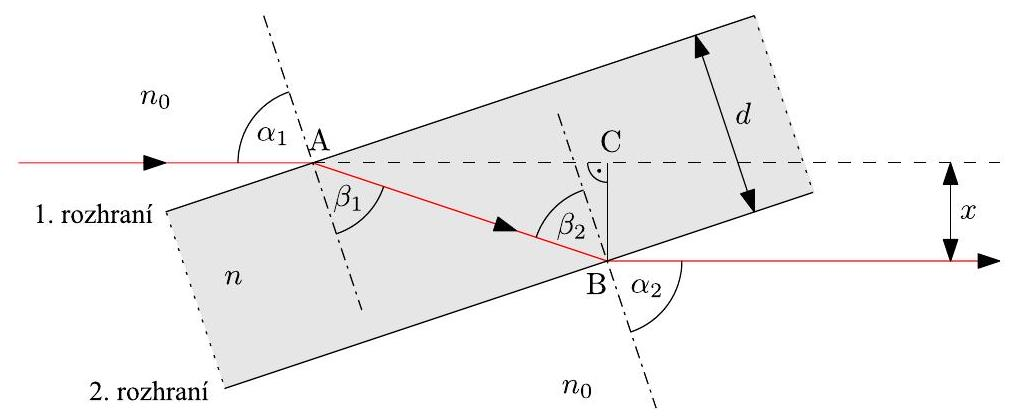
\includegraphics[max width=0.9\linewidth]{2024_11_19_160a1389244899f42734g-5}
		\end{center}
		
		Obrázek 4: Průchod světla planparalelní deskou.
		
		Odchylka $x$ vstupujícího a vystupujícího paprsku je
		
		\begin{equation}
			x=|B C|=|A B| \sin (\alpha-\beta)
		\end{equation}
		
		
		Úpravou a použitím vztahů
		
		
		\begin{equation}
			\cos \beta=\sqrt{1-\sin ^{2} \beta}, \quad \sin (\alpha-\beta)=\sin \alpha \cos \beta-\cos \alpha \sin \beta
		\end{equation}
		
		obdržíme z 11-14 vztah pro odchylku paprsků,
		
		
		\begin{equation}
			x=\left(1-\frac{n_{0} \cos \alpha}{\sqrt{n^{2}-n_{0}^{2} \sin ^{2} \alpha}}\right) d \sin \alpha
		\end{equation}
		
		Z tohoto vztahu můžeme určit index lomu skla za předpokladu, že $\alpha \neq 0$ :
		
		\begin{equation}
			n=n_{0} \sqrt{\sin ^{2} \alpha+\left(1-\frac{x}{d \sin \alpha}\right)^{-2} \cos ^{2} \alpha}
		\end{equation}
		
		\section*{Experiment}
		Pro měření úhlu dopadu, posuvu $x$ nebo úhlu deviace použijeme goniometr, jehož schéma a fotografie jsou na obrázku 5. Goniometr obsahuje kruhovou stupnici ST, po které se pohybují tři ramena: R1 se zdrojem, kterým je laserová dioda $\mathrm{L}, \mathrm{R} 2 \mathrm{~s}$ detektorem D tvořeným Si fotodiodou a R3 se stolečkem S pro vzorek umístěným ve středu kruhu. Na stolek klademe zkoumanou planparalelní desku (nebo hranol). Detektorem lze posunovat šroubem ve směru $x$ kolmo na rameno R2.\\
		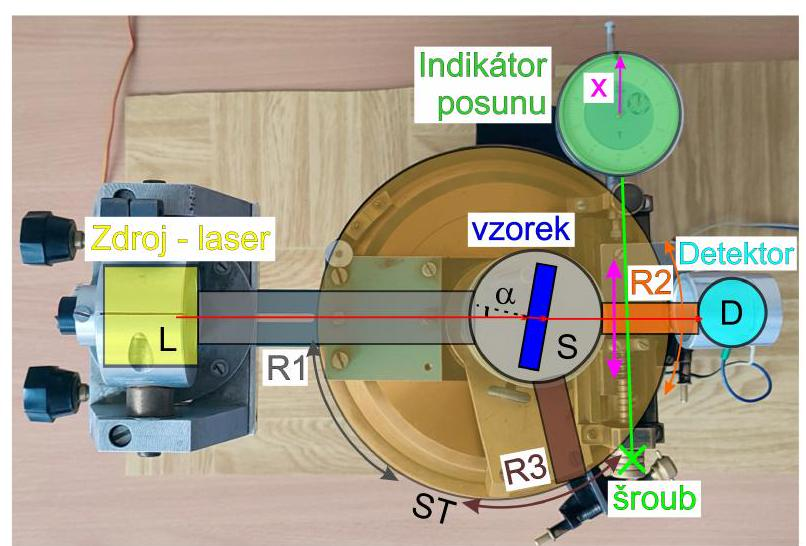
\includegraphics[max width=0.9\linewidth, center]{2024_11_19_160a1389244899f42734g-5(1)}
		
		Obrázek 5: Experimentální uspořádání pro měření průchodu světla planparalení deskou a hranolem.
		
		Posuv se měří pomocí indikátoru v podobě číselníkového úchylkoměru. Úhel dopadu $\alpha$ určujeme z polohy ramen R1 a R3, úhel deviace výstupního paprsku $\delta$ z polohy ramen R1 a R2 (pro desku je $\delta=0$ ).
		
		Před měřením je třeba nastavit stolek $S$ tak, aby paprsek dopadal kolmo na měřenou planparalelní desku nebo hranol. Dosáhne se toho pomocí tří stavících šroubů pod stolečkem. Kolmost dopadajícího paprsku na lámavou plochu poznáme podle chodu zpětně odraženého paprsku: oba paprsky musí mít totožnou dráhu - sledujeme stopu odraženého paprsku u výstupního otvoru zdroje. (Pokud použijeme hranol, tak jeho lámavý úhel je $60^{\circ}$.)
		
		Úhel dopadu měňte otáčením stolečku S ramenem R3. Správnou polohu detektoru poznáte podle maximální hodnoty fotoproudu, který méřte digitálním ampermetrem.
		\section{Měření}
		\subsection{Měření odrazivosti dielektrika}
		Po adjustaci goniometru provádíme měření pro S a P polarizaci v rozmezí 26-85°. Intenzitu zdroje (tj. mimo odraz) měříme přímým namířením laseru na detektor bez překážek v trajektorii, znovu pro S i P polarizaci. Získáváme:
		\begin{figure}[H]
			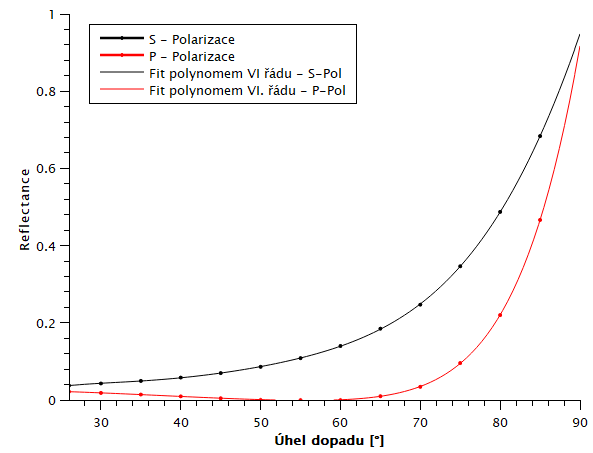
\includegraphics[width=1\linewidth, center]{Reflectance}
		\end{figure}
		
		Z formule (8),(9) získáváme hodnotu
		\begin{equation}
			n = 1.417 \pm 0.006
		\end{equation}
		
		
		Při hledání lokálního extrému - tj. hodnoty Brewsterova úhlu - proložíme naměřené hodnoty polynomem a hledáme jeho kořen. Získáváme hodnotu
		\begin{equation}
			\varphi_{B} = 56.1794 °
		\end{equation}
		Z formule (4) tedy získáváme index lomu:
		\begin{equation}
			n = \tan \varphi_B = 1.492
		\end{equation}
		
		Nyní můžeme průběh reflektance se získanými úhly srovnat:
		\begin{figure}[H]
			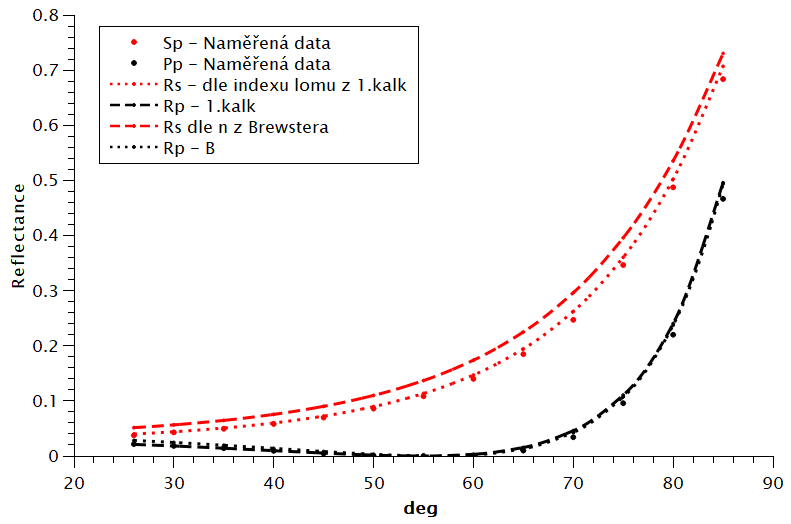
\includegraphics[width = 0.9\linewidth, center]{Srovnani}
		\end{figure}
		Vidíme, že se hodnoty získané z výsledku (18) našim naměřeným hodnotám blíží více.
		Totéž můžeme využitím formule (7) provést pro nepolarizované světlo. Získáváme:
		\begin{figure}[H]
			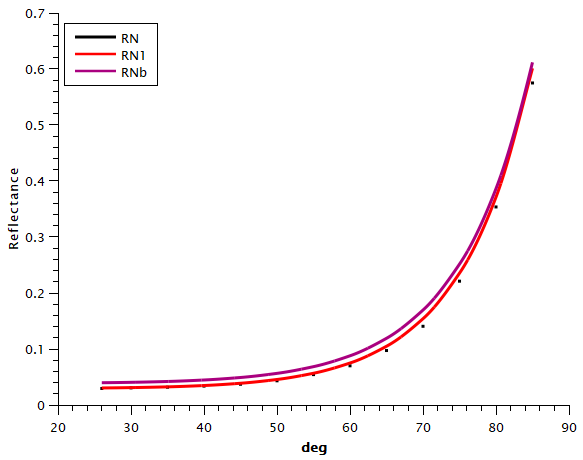
\includegraphics[width = 0.9\linewidth, center]{Rn}
		\end{figure}
		\subsection{Průchod světla planparalelní deskou}
		Pro desku o tloušťce $d = 20.147 \pm 0.008 \,\rm mm$ získáváme hodnoty, ze kterých kalkulujeme index lomu materiálu. Získáváme:
		\begin{center}
			\begin{tabular}{|l|l|l|}
			\hline
			$\varphi _i$ [°] & x [mm] & n                \\ \hline
			10               & 1.135  & 1.468 \\ \hline
			15               & 1.75   & 1.477 \\ \hline
			20               & 2.4    & 1.482 \\ \hline
			25               & 3.1    & 1.487  \\ \hline
			30               & 3.875  & 1.494 \\ \hline
			35               & 4.69   & 1.493 \\ \hline
			40               & 5.6    & 1.495 \\ \hline
			45               & 6.63   & 1.500 \\ \hline
			50               & 7.7    & 1.494 \\ \hline
			55               & 8.9    & 1.490 \\ \hline
		\end{tabular}
		\end{center}
		Pro hodnotu indexu lomu tedy získáváme\\ $n = 1.488 \pm 0.003$
		Z této hodnoty pomocí formule (16) můžeme získat teoreticky správné hodnoty $x$ a tyto hodnoty s naměřenými daty porovnat:
		\begin{figure}[H]
			\includegraphics[width = 0.9\linewidth, center]{Srovnani2}
		\end{figure}
		Vidíme, že odchylky jsou minimální.
		
		\section{Závěr}
		Podařilo se nám splnit veškeré zadané úkoly a získat hodnoty hledaných veličin. Je třeba myslet na to, že skutečné hodnoty nevíme. Byť malými, ale stále přítomnými imperfekcemi našeho postupu v našich hodnotách rozhodně vzešly jisté odchylky od skutečné hodnoty. Nelze tudíž brát naměřené hodnoty a teoretickou kalkulaci, která vzešla z těchto hodnot, jako porovnání výsledků s něčím absolutně korektním, spíše stojí za to se zaměřit na srovnání průběhů jako celku. Nelze říci, že je u indexu lomu spočítaného z refrakce hodnota (18) přesnější než (20), jelikož její refrakční křivka je bližší naší naměřené. Naopak jsme přesvědčeni, že metoda Brewsterova úhlu nám dala přesnější údaj, jelikož jsme hledali pouze lokální minimum, kde nezáleželo na "kalibraci" intenzitou dopadajícího světla. Je možné, že jsme v tomto značně biasovani, jelikož nám řešení pro Brewsterův úhel vyšlo extrémně blízko indexu lomu PMMA (plexiskla, akrylátového skla). 
	
		

		
		
		
		
		
		% Nakonec nezapomeňte projet text programem vlna nebo vlnka, např.
		% 	vlna -m -l -n mojeuloha.tex
		% nebo zkontrolovat a opravit jednopísmenné předložky na koncích řádků ručně.
	\end{multicols}
\end{document}
